
\paragraph{Utility} 
\textbf{Level 0 } 
\begin{tabular}{ m{4cm}m{3cm}m{6cm} } 
	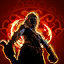
\includegraphics[width=4cm]{../Pictures/Gameplay/Spells/Icon/spell_icon.png} & \textbf{Lumos} & Illuminates the tip of the caster's wand, allowing the caster to see in the dark. The spell ends if you cast it again or dismiss it as an action.\\ 
	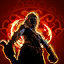
\includegraphics[width=4cm]{../Pictures/Gameplay/Spells/Icon/spell_icon.png} & \textbf{Reparo} & Seamlessly repairs broken objects. This spell repairs a single break or tear in an object you touch, such as a broken chain link, two halves of a broken key, a torn cloak, or a leaking wineskin \\ 
	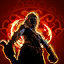
\includegraphics[width=4cm]{../Pictures/Gameplay/Spells/Icon/spell_icon.png} & \textbf{Accio} &  Summons an object towards the caster. Describe or name an object that is familiar to you. \\ 
\end{tabular}

\textbf{Level 1 } 
\begin{tabular}{ m{4cm}m{3cm}m{6cm} } 
	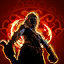
\includegraphics[width=4cm]{../Pictures/Gameplay/Spells/Icon/spell_icon.png} & \textbf{Wingardium Leviosa} & Makes objects fly, or levitate. The target can move only by pushing or pulling against a fixed object or surface within reach (such as a wall or a ceiling), which allows it to move as if it were climbin  \\ 
	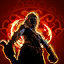
\includegraphics[width=4cm]{../Pictures/Gameplay/Spells/Icon/spell_icon.png} & \textbf{Fumos} & roba \\ %todo
\end{tabular}
\textbf{Level 3} 
\begin{tabular}{ m{4cm}m{3cm}m{6cm} } 
	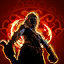
\includegraphics[width=4cm]{../Pictures/Gameplay/Spells/Icon/spell_icon.png} & \textbf{Alohomora} & Unlocks doors and other locked objects. Choose an object that you can see within range. The object can be a door, a box, a chest, a set of manacles, a padlock, or another object that contains a mundane or magical means that prevents access. \\ 
   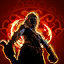
\includegraphics[width=4cm]{../Pictures/Gameplay/Spells/Icon/spell_icon.png} & \textbf{Colloportus} &  Locks doors and all things that can be locked. You touch a closed door, window, gate, chest, or other entryway, and it becomes locked for the duration. \\ 
\end{tabular}
\textbf{Level 5} 
\begin{tabular}{ m{4cm}m{3cm}m{6cm} } 
	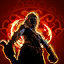
\includegraphics[width=4cm]{../Pictures/Gameplay/Spells/Icon/spell_icon.png} & \textbf{Revelio} & Reveals secrets about a person or object.  \\ %todo
	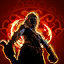
\includegraphics[width=4cm]{../Pictures/Gameplay/Spells/Icon/spell_icon.png} & \textbf{Transfiguration} & Transforms a teacup into a tortoise.  An unwilling creature must make a Wisdom saving throw to avoid the effect. The spell has no effect on a shapechanger or a creature with 0 hit points. The transformation lasts for the duration, or until the target drops to 0 hit points or dies. The new form can be any beast whose challenge rating is equal to or less than the target's (or the target's level, if it doesn't have a challenge rating). The target's game statistics, including mental ability scores, are replaced by the statistics of the chosen beast. It retains its alignment and personality.\\ 
\end{tabular}
\textbf{Level 7} 
\begin{tabular}{ m{4cm}m{3cm}m{6cm} } 
	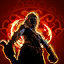
\includegraphics[width=4cm]{../Pictures/Gameplay/Spells/Icon/spell_icon.png} & \textbf{Apparate} & Magically transports the caster to another location instantaneously.  \\ &todo
\end{tabular}
\textbf{Level 8} 
\begin{tabular}{ m{4cm}m{3cm}m{6cm} } 
	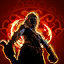
\includegraphics[width=4cm]{../Pictures/Gameplay/Spells/Icon/spell_icon.png} & \textbf{Portkey} & Turns an object into a portkey. . You and any creatures that teleport with you appear in the nearest unoccupied space to the spot you designated when you prepared your sanctuary (see below). If you cast this spell without first preparing a sanctuary, the spell has no effect. \\ 
\end{tabular}


\pagebreak











